%
% File acl2017.tex
%
%% Based on the style files for ACL-2015, with some improvements
%%  taken from the NAACL-2016 style
%% Based on the style files for ACL-2014, which were, in turn,
%% based on ACL-2013, ACL-2012, ACL-2011, ACL-2010, ACL-IJCNLP-2009,
%% EACL-2009, IJCNLP-2008...
%% Based on the style files for EACL 2006 by 
%%e.agirre@ehu.es or Sergi.Balari@uab.es
%% and that of ACL 08 by Joakim Nivre and Noah Smith

\documentclass[11pt,a4paper]{article}
\usepackage[hyperref]{acl2017}
\usepackage{times}
\usepackage{latexsym}
\usepackage{graphicx}
\usepackage{amsmath}
\usepackage{amssymb}
\usepackage{url}

\aclfinalcopy % Uncomment this line for the final submission
%\def\aclpaperid{***} %  Enter the acl Paper ID here

%\setlength\titlebox{5cm}
% You can expand the titlebox if you need extra space
% to show all the authors. Please do not make the titlebox
% smaller than 5cm (the original size); we will check this
% in the camera-ready version and ask you to change it back.

% \newcommand\BibTeX{B{\sc ib}\TeX}

\title{Neural Knowledge Acquisition from Joint Representation of Knowledge Graph and Text}

% \author{First Author \\
%   Affiliation / Address line 1 \\
%   Affiliation / Address line 2 \\
%   Affiliation / Address line 3 \\
%   {\tt email@domain} \\\And
%   Second Author \\
%   Affiliation / Address line 1 \\
%   Affiliation / Address line 2 \\
%   Affiliation / Address line 3 \\
%   {\tt email@domain} \\}

% \date{}

\begin{document}
\maketitle

\begin{abstract}
  Joint learning methods in Natural Language Processing (NLP) have usually focused on some similar tasks so that complementary linguistic features of morphology, syntax and semantics from different models would benefit each other. In this paper, we propose a novel joint learning framework for both knowledge graph completion (KGC) and relation extraction (RE). By learning representations of KGs and text within a unified semantic space, structural KG features and rich flexible textual features enhance models together. The joint mechanism enables us to take both KGs and plain text into consideration at the same time and perform KGC and RE more accurately. In experiments, we evaluate our joint learning model on three classical tasks including relation extraction, entity prediction and relation prediction. The experiment results show that our joint model can significantly and consistently improve the performances on the three tasks as compared with other baselines without joint learning. The source code of our joint model would be released in the public then.
\end{abstract}


\section{Introduction}
\label{intro}

People construct various large-scale knowledge graphs (KGs) to organize structural knowledge about the world, such as WordNet \cite{miller1995wordnet}, YAGO \cite{suchanek2007yago}, DBPedia \cite{auer2007dbpedia}, Freebase \cite{bollacker2008freebase}, Knowledge Vault \cite{dong2014knowledge} and Wikidata\cite{vrandevcic2014wikidata}. A typical knowledge graph is a multiple-relational directed graph with nodes corresponding to entities, and edges corresponding to relations between these entities. The facts in KGs are usually recorded as a set of relational triples ($h$, $r$, $t$) with $h$, $t$ indicating \emph{head}, \emph{tail} entities and $r$ indicating the relation between $h$ and $t$, e.g., (\emph{Mark Twain}, \texttt{PlaceOfBirth}, \emph{Florida}). Owing to rich and structural inner information, KGs are playing an important role in numerous applications especially in question answering and web searching.

\begin{figure}[]
\centering
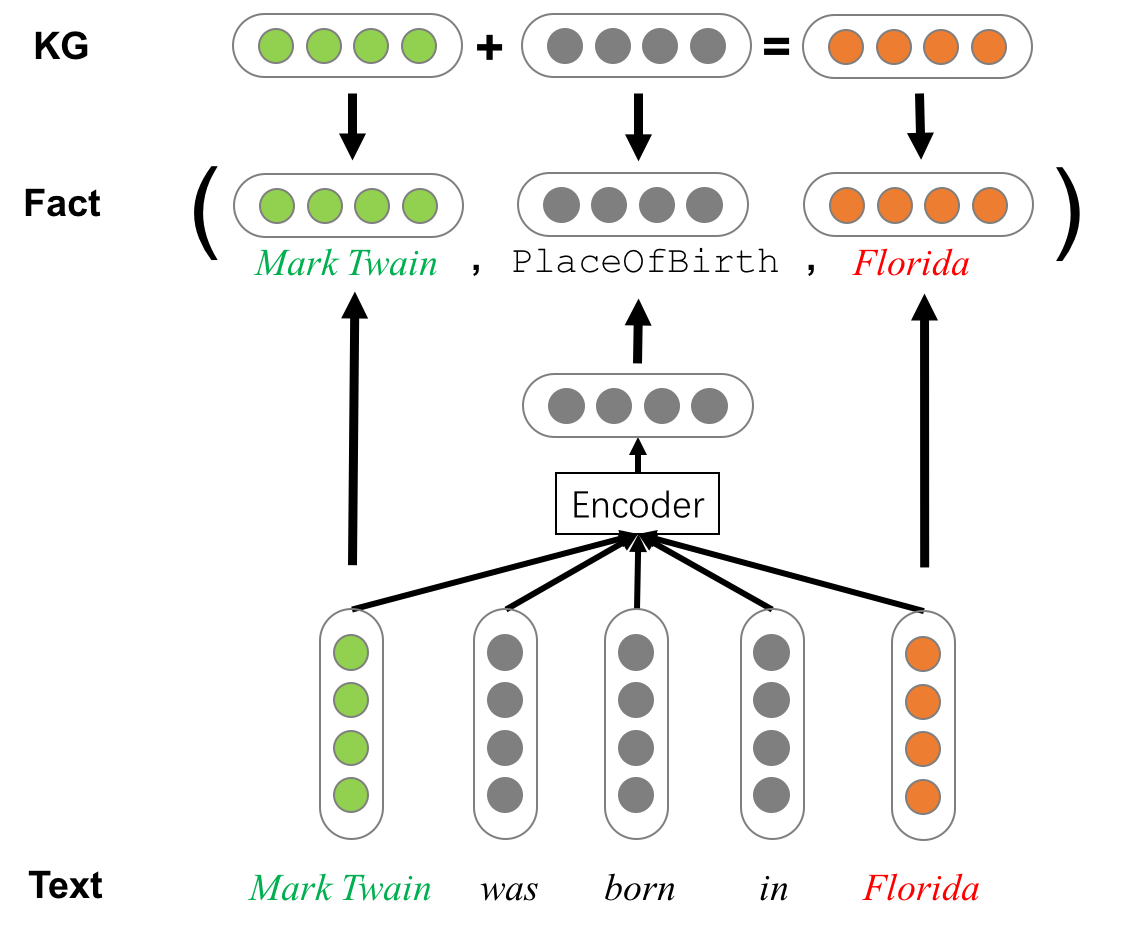
\includegraphics[width=\columnwidth]{gg1.png}
\caption{The framework of joint representation learning of the knowledge graph and text.}
\label{fig:joinglearning}
\end{figure}

However, typical large-scale KGs are usually far from complete. The task of knowledge graph completion (KGC) aims to enrich KGs with novel facts. Based on the network structure of KGs, many graph-based methods have been proposed to mine novel facts between entities \cite{lao2011random,lao2010relational}. Many efforts are also devoted to extract relational facts from plain text \cite{surdeanu2012multi,riedel2013relation,min2013distant,zeng2014relation,zeng2015distant,dos2015classifying,lin2016neural} for the task of relation extraction (RE). Though the two tasks are similar, the past approaches cannot jointly take both KGs and plain text into consideration.

In recent years, neural-based knowledge representation has been proposed to encode both entities and relations into a low-dimensional space, which are capable to find novel facts \cite{bordes2013translating,wang2014transh,lin2015learning,ji2015knowledge,he2015learning,xiao2015transg,ji2016knowledge}. More importantly, neural models enable us to conduct joint representation learning of KGs and text within a unified semantic space, and perform KGC and RE more accurately.

Some pioneering works have been done. For example, \cite{wang2014knowledge} performs joint learning simply considering alignment between words and entities, and \cite{toutanova2015representing} extracts textual relations from plain text using dependency parsing to enhance relation embeddings. These works either consider only partial information in plain text (only entity mentions in \cite{wang2014knowledge,xie2016representation,wu2016knowledge,zeng2016incorporating} and only textual relations in \cite{toutanova2015representing}), or rely on complicated linguistic analysis (dependency parsing in \cite{toutanova2015representing}) which may bring inevitable parsing errors.

To address these issues, we propose a novel framework for joint representation learning. As shown in Figure \ref{fig:joinglearning}, the framework is expected to take full advantages of both KGs and text via complicated alignments with respect to words, entities and relations. Moreover, our method applies deep neural networks with a knowledge-attention mechanism instead of native linguistic analysis to encode the semantics of sentences, which is especially capable of modeling large-scale and noisy Web text. 

We conduct experiments on a real-world dataset whose KG extracted from Freebase and text derived from the New York Times corpus. We evaluate our method on the tasks of KGC (entity prediction and relation prediction) and RE (relation extraction from text). Experiment results demonstrate that, our method can effectively perform joint representation learning and obtain more informative knowledge and text representation, which significantly outperforms other baseline methods.

\section{Related Work}
\label{sec:related}
Our work relates to representation learning of KGs, words, textual relations and neural networks with attention. Related works are reviewed as follows.

\textbf{Representation Learning of KGs.} A variety of approaches have been proposed to encode both entities and relations into a continuous low-dimensional space. Inspired by \cite{mikolov2013distributed}, TransE \cite{bordes2013translating} regards the relation $r$ in each fact ($h$, $r$, $t$) as a translation from $h$ to $t$ within the low-dimensional space, i.e., $\textbf{h} + \textbf{r} = \textbf{t}$, where $\textbf{h}$ and $\textbf{t}$ are entity embeddings and $\textbf{r}$ is relation embedding. Despite of its simplicity, TransE achieves the state-of-the-art performance of representation learning for KGs, especially for large-scale and sparse KGs. Hence, we simply incorporate TransE in our method to handle representation learning for KGs.

Note that, our method is also flexible to incorporate extension models of TransE, such as TransH \cite{wang2014transh}, TransR \cite{lin2015learning}, TransD \cite{ji2015knowledge} and TranSparse \cite{ji2016knowledge}, which is not the focus of this paper and will be left as our future work.

\textbf{Representation Learning of Words.} Given a text corpus, we can learn word representations without supervision. The learning objective is defined as the likelihood of predicting its context words of each word or vice versa \cite{mikolov2013distributed}. Continuous Bag-of-Words (CBOW) \cite{mikolov2013efficient} and Skip-Gram \cite{mikolov2013linguistic} are state-of-the-art methods for word representation learning. The learned word embeddings can capture both syntactic and semantic features of words derived from plain text corpus. As reported in many previous works, deep neural network will benefit significantly if being initialized with pre-trained word embeddings \cite{erhan2010does}. In this work, we apply Skip-Gram for word representation learning, which serves as initialization for joint representation learning of text and KGs.

\textbf{Representation Learning of Textual Relations.} Many works aim to extract relational facts from large-scale text corpus \cite{mintz2009distant,riedel2010modeling}. This indicates textual relations between entities are contained in plain text. In recent years, deep neural models such as convolutional neural networks (CNN) have been proposed to encode semantics of sentences to identify relations between entities \cite{zeng2014relation,dos2015classifying,zeng2015distant,lin2016neural}. As compared to conventional models, neural models are capable to accurately capture textual relations between entities from text sequences without explicitly linguistic analysis, and further encode into continuous vector space. Hence, in this work we apply CNN to embed textual relations and conduct joint learning of text and KGs with respect to relations.

Many neural models such as recurrent neural networks (RNN) \cite{zhang2015relation} and long-short term memory networks (LSTM) \cite{xu2015classifying,miwa2016end} have also been explored for RE. These models can also be applied to perform representation learning for textual relations. However, shortcomings of RNN in long-term dependencies and time efficiency make us prefer CNN for representation of textural relations.

\textbf{Neural Networks with Attention.} \cite{bahdanau2014neural} first proposed the attention mechanism in neural networks for machine translation. The attention mechanism is implemented to select the most relevant and important hidden features encoded from the original sentence to better decode the target sentence. Due to the ability to catch key points in text, many attention models has been proposed for several NLP tasks, such as entity type classification \cite{shimaoka2016attentive}, machine reading \cite{hermann2015teaching,dhingra2016gated,sordoni2016iterative}. \cite{yang2016hierarchical} proposed a hierarchical attention network over sentences for document classification, and further more, \cite{lin2016neural} use the sentence selective attention model for RE. In this paper, we propose a multilevel-attention mechanism for both words and sentences under knowledge KG guidance.

\section{The Framework}
In this section we introduce the framework of joint representation learning, starting by notations and definitions.

\subsection{Notations and Definitions}

We denote a knowledge graph as $G = \{E, R, T\}$, where $E$ indicates a set of entities, $R$ indicates a set of relation types, and $T$ indicates a set of fact triples. Each triple $(h, r, t) \in T$ indicates there is a relation $r \in R$ between $h \in E$ and $t \in E$.

We denote a text corpus as $D$ and its vocabulary as $V$, containing all words, phrases and entity mentions. In the corpus $D$, each sentence is denoted as a word sequence $s = \{x_1, \ldots, x_n\}, x_i \in V$, and $n$ is the sentence length.

For entities, relations and words, we use the bold face to indicate their corresponding low-dimensional vectors. For example, the embeddings of $h, t \in E$, $r \in R$ and $x \in V$ are $\mathbf{h}, \mathbf{t}, \mathbf{r}, \mathbf{x} \in \mathbb{R}^{k_w}$ respectively, where $k_w$ is the embedding dimension.


\subsection{Joint Learning Method}
As mentioned in Section \ref{sec:related}, representation learning methods have been proposed for knowledge graphs and text corpora respectively. In this work, we propose a joint learning framework for both the KG and text.

In this framework, we aim to jointly learn representations of entities, relations and words. With denoting all these representations as model parameters $\theta = \{\theta_E, \theta_R, \theta_V\}$, the framework aims to find optimized parameters

\begin{equation}
\hat{\theta} = \mathop{\arg\max}_{\theta} P(G, D | {\theta}),
\end{equation}

where $\theta_E, \theta_R, \theta_V$ are parameters for entities, relations and words respectively. $P(G, D | {\theta})$ is the conditional probability defined over the knowledge graph $G$ and the text corpus $D$ given the parameters $\theta$. The conditional probability can be further decomposed as:


\begin{align}
\label{eq:topeq}
P(G,D|{\theta}) = P(G|{\theta_E,\theta_R})P(D|{\theta_V}) \\\nonumber
= \prod_{(h,r,t) \in G}P((h, r, t)|{\theta_E, \theta_R}) \prod_{s \in D}P((s, r_s)|{\theta_V}), \\\nonumber
\end{align}

where $P((h, r, t)|{\theta_E,\theta_R})$ denotes the conditional probability of relational triples $(h, r, t)$ in the knowledge graph $G$ and $P((s, r_s)|{\theta_V})$ denotes the conditional probability of sentences and their corresponding textual relations $(s, r_s)$ in the text corpus $D$.

$P(G|\theta_E, \theta_R)$ is responsible to learn representations of both entities and relations from the knowledge graph $G$. This part will be introduced in detail in Section \ref{sec:kg}.

$P(D|{\theta_V})$ is responsible to learn representations of sentence words as well as textual relations from the text corpus $D$. It is straightforward to learn word representations from text as discussed in Section \ref{sec:related}. Since entities and relations are not explicitly shown in text, we have to identify entities and relations in text to support information exchange between entities and words, relations and textual relations. The process is realized by entity-text alignment and relation-text alignment.

\textbf{Entity-Text Alignment.} Many entities are mentioned in text. Due to the complex polysemy of entity mentions (e.g., an entity name Washington in a sentence could be indicating either a person or a location), it is non-trivial to build entity-text alignment. The alignment can be built via entity linking techniques or anchor text information. In this paper, we simply use the anchor text annotated in articles to build the alignment between entities in $E$ and entity mentions in $V$. We will share the aligned entity representations in $\theta_E$ to corresponding entity mentions in $\theta_V$.

\textbf{Relation-Text Alignment.} As mentioned in Section \ref{sec:related}, textual relations can be extracted from text. Hence, relation representation can also be learned from plain text. Inspired by the idea of distant supervision, for a relation $r \in R$, we collect all entity pairs $Pair_{r} = \{(h, t)\}$ connected by $r$ in the KG. Afterwards, for each entity pair in $Pair_{r}$, we extract all sentences that contain the both entities from $D$, and regard them as the positive instances of the relation $r$. We can further apply deep neural networks to encode the semantic of these sentences into the corresponding relation representation. The process will be introduced in detail in Section \ref{sec:relation}.

In summary, the framework enables joint representation learning of both entities and relations by taking full advantages of both KG and text. The learned representations are expected to be more informative and robust, which will be verified in experiments.



\subsection{Representation Learning of KGs}
\label{sec:kg}

We aim to embed entities and relations to capture the correlations between them. When learning from relational triples, we usually optimize the conditional probability $P(h|(r, t),{\theta_E, \theta_R})$, $P(t|(h, r),{\theta_E, \theta_R})$, and $P(r|(h, t),{\theta_E, \theta_R})$ instead of $P((h, r, t)|{\theta_E, \theta_R})$

For each entity pair $(h, t)$ in a KG $G$, we define their latent relation embedding $\mathbf{r}_{ht}$ as a translation from $\mathbf{h}$ to $\mathbf{t}$, which can be formalized as:
\begin{equation}
\textbf{r}_{ht} = \textbf{t} - \textbf{h}.
\end{equation}
Meanwhile, each triple $(h, r, t) \in T$ has an explicit relation $r$ between $h$ and $t$. Hence, we can define the scoring function for each triple as follows:
\begin{equation}
f_r(h, t) = b1 - \lVert \textbf{r}_{ht} - \textbf{r} \rVert_2 = b1 - \lVert (\textbf{t} - \textbf{h}) - \textbf{r}  \rVert_2.
\end{equation}
where b1 is a bias constant. This indicates that, for each triple $(h, r, t)$ in $T$, we expect $\textbf{h} + \textbf{r} \approx \textbf{t}$.

Based on the above scoring function, the conditional probability can be formalized over all triples in $T$ as follows:

\begin{align}
P(h|(r, t),{\theta_E, \theta_R}) = \frac{exp(f_r(h, t))}{\sum_{h' \in E} exp(f_r(h', t))}
\end{align}

We also define $P(t|(h, r), {\theta_E, \theta_R})$ and $P(r|(h, t),{\theta_E, \theta_R})$ in the same way by choosing corresponding normalization terms respectively. In fact, this representation objective is consistent with TransE \cite{bordes2013translating}. Other knowledge representation (KR) models evolved from TransE can also be easily adopted in this framework by changing the scoring function, such as TransH \cite{wang2014transh}, TransR \cite{lin2015learning}, TransD \cite{ji2015knowledge} and TranSparse \cite{ji2016knowledge}. 

\subsection{Representation Learning of Textual Relations}
\label{sec:relation}

Given a sentence containing two entities, the words in the sentence usually expose implicit features of the textual relation between the two entities. As shown in \cite{zeng2014relation,toutanova2015representing,lin2016neural}, the textual relations can be learned with deep neural networks and encoded in the low-dimensional semantic space.

We follow \cite{zeng2014relation,toutanova2015representing,lin2016neural} and apply convolutional neural networks (CNN) to model textual relations from text. 

% CNN is an efficient neural model widely used in image processing, which has been verified to be also effective for many NLP tasks such as part-of-speech tagging, named entity recognition and semantic role labeling.

\begin{figure*}[!htbp]
\centering
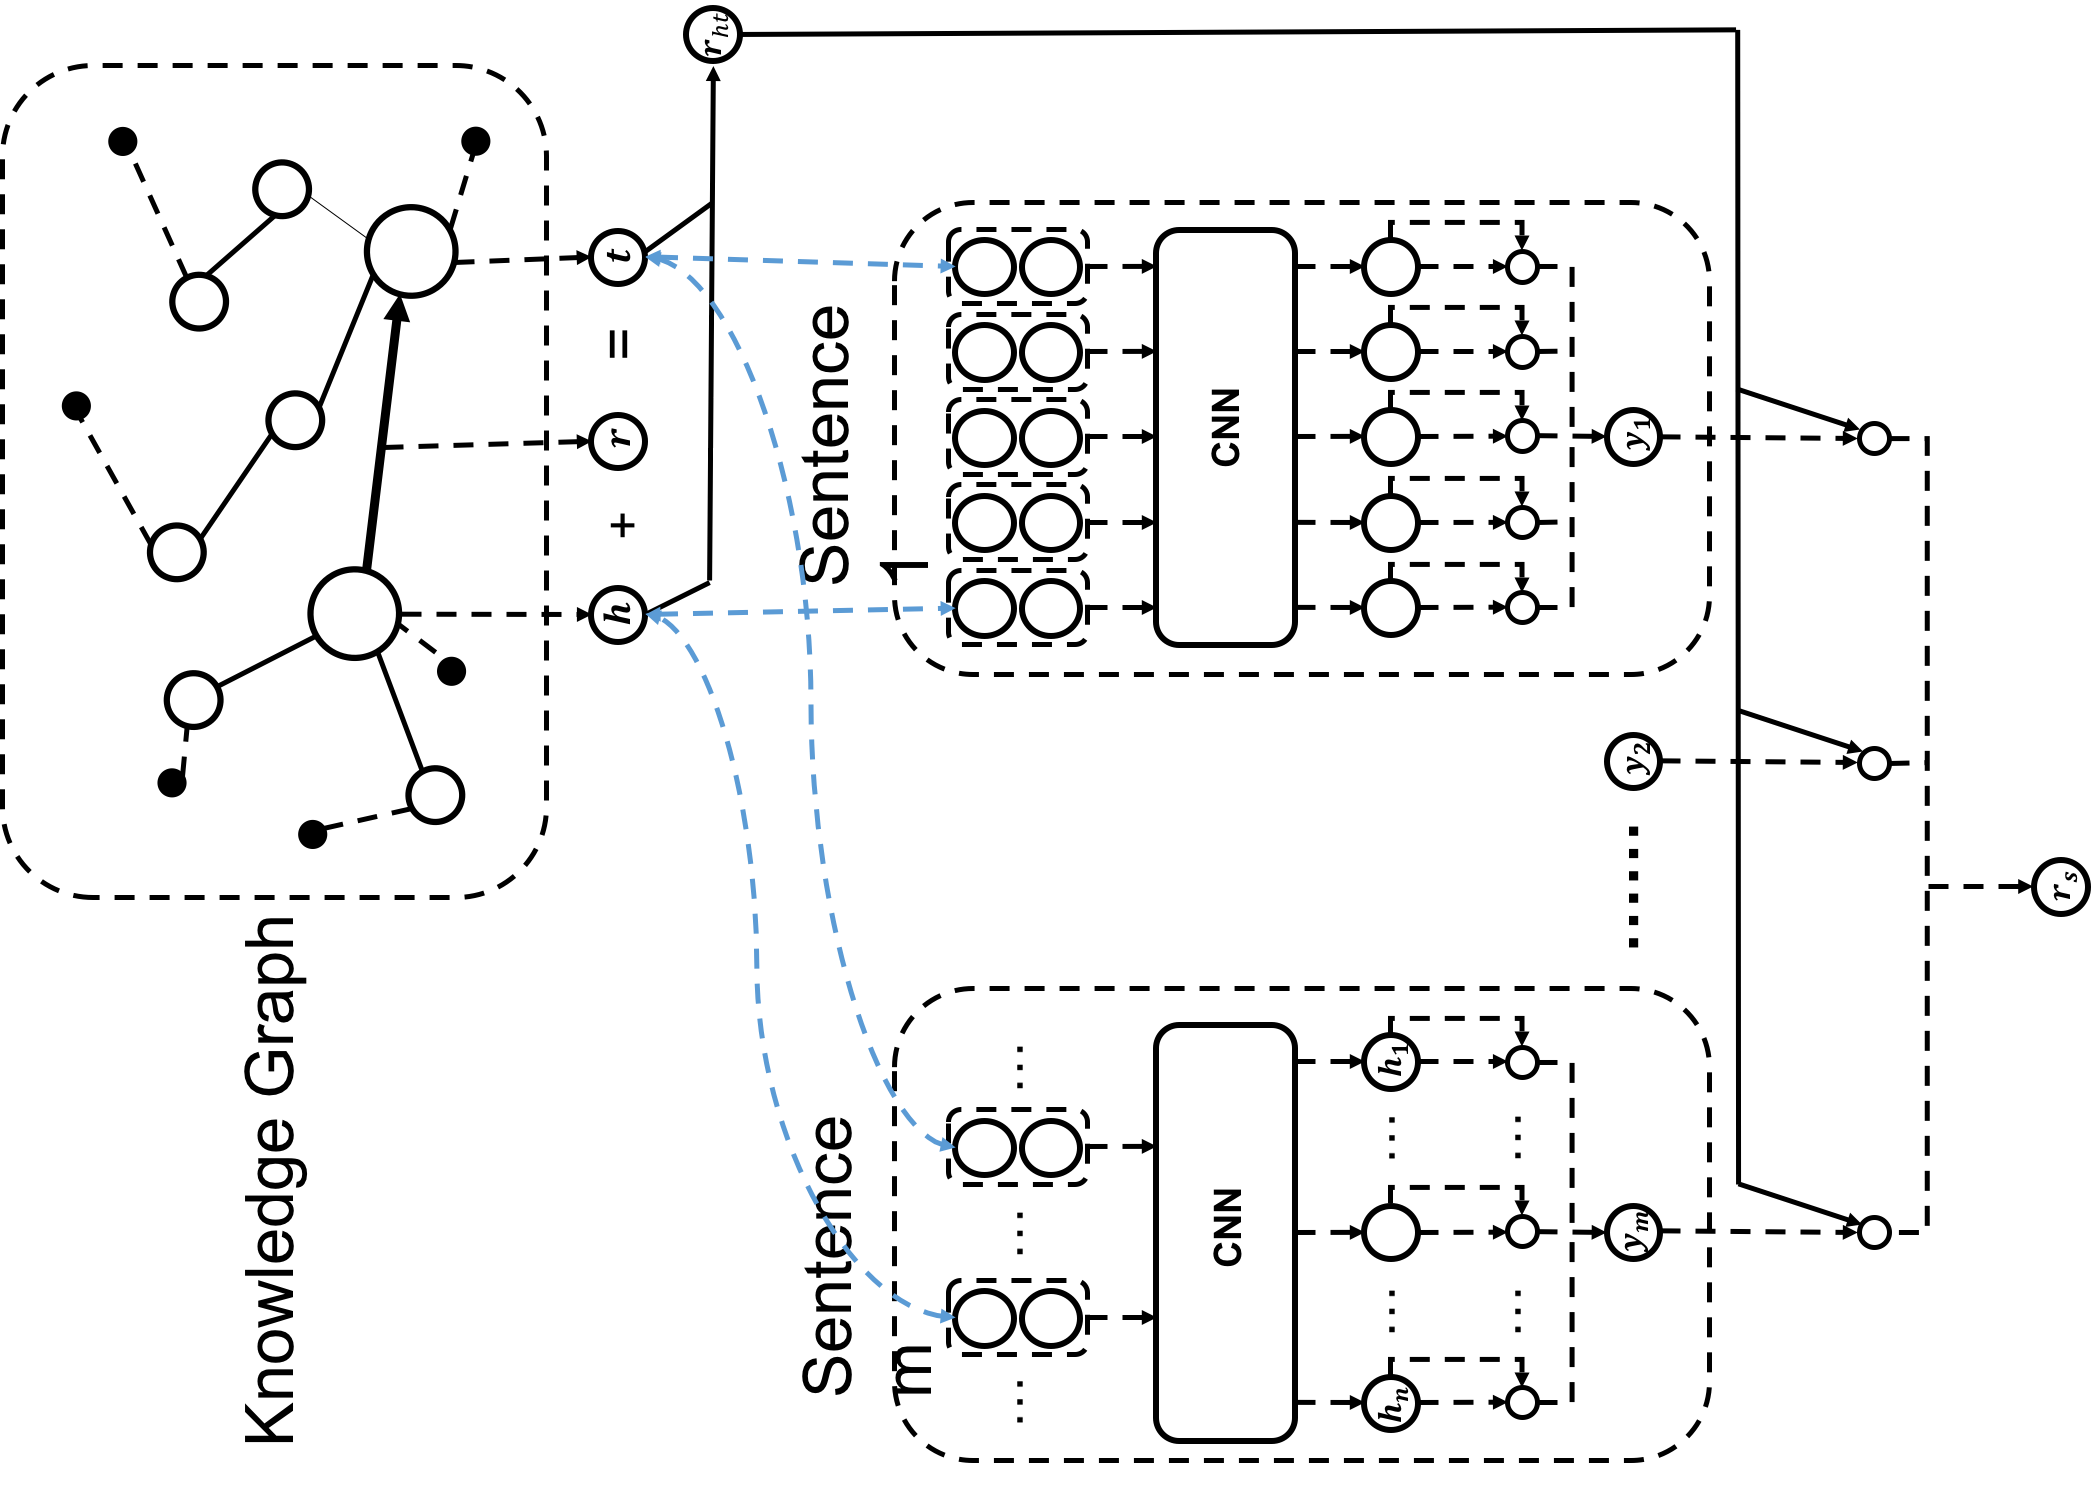
\includegraphics[width=0.9\textwidth]{cnn.png}
\caption{Convolutional neural networks for representation learning of textual relations.}
\label{fig:cnn}
\end{figure*}


\subsubsection{Overall Architecture}

Figure \ref{fig:cnn} depicts the overall architecture of CNN for modeling textual relations. For a sentence $s$ containing $(h, t)$ with a relation $r_s$, the architecture takes word embeddings $\mathbf{s} = \{\mathbf{x}_1, \ldots, \mathbf{x}_n \}$ of the sentence $s$ as input, and after passing through two layers within CNN, outputs the embedding of the textual relation $\mathbf{r}_{s}$. Our method will further learn to get the scoring function through a softmax layer as follows,

\begin{equation}
f(s) = \mathbf{M}\mathbf{r}_{s} + \mathbf{d},
\label{eq:cnn_distance}
\end{equation}

where $\mathbf{d} \in \mathbb{R}^{\|R\|}$ is a bias vector and $\mathbf{M}$ is the representation matrix to calculate the relation scorings. Finally we define the conditional probability $P((s, r_s)|{\theta_V})$ 

\begin{equation}
P((s, r_s)|{\theta_V}) = \frac{exp(f_{r_s}(s))}{\sum_{r \in R} exp(f_{r}(s))}
\end{equation}

In this paper, our CNN contains an input layer, a convolution layer and a multilevel-attention mechanism. All of these are introduced in detail as follows.

\subsubsection{Input Layer}
Given a sentence $s$ made up of $n$ words $s = \{ x_1, \ldots , x_n\}$, the input layer transforms the words of $s$ into corresponding word embeddings $\mathbf{s} = \{ \mathbf{x}_1, \ldots , \mathbf{x}_n \}$. For a word $x_i$ in the given sentence, its input embedding $\mathbf{x}_i$ is composed of two real-valued vectors: its textual word embedding $\mathbf{w}_i$ and its position embedding $\mathbf{p}_{i}$.

Textual word embeddings encode the semantics of the corresponding words, which are usually pre-trained from plain text via word representation learning, as introduced in Section \ref{sec:detail}.

Word position embeddings (WPE) is originally proposed in \cite{zeng2014relation}. WPE is a position feature indicating the relative distances of the given word to the marked entities in the sentence. As shown in Figure \ref{fig:cnn}, the relative distances of the word \emph{born} to the entities \emph{Mark Twain} and \emph{Florida} are $-2$ and $+2$ respectively. We map each distance to a vector of dimension $k_p$ in the continuous latent space. Given the word $x_i$ in the sentence $s$, the word position embedding is $\mathbf{p}_i = [\mathbf{p}^h_i, \mathbf{p}^t_i]$, where $\mathbf{p}^h_i$ and $\mathbf{p}^t_i$ are vectors of distances to the head entity and tail entity respectively.

We simply concatenate textual word embeddings and word position embeddings to build the input for CNN:
\begin{equation}
\mathbf{s} = \{[\mathbf{w}_1;\mathbf{p}_1],\ldots, [\mathbf{w}_n;\mathbf{p}_n]\}.
\end{equation}

\subsubsection{Convolution Layer}
By taking $\mathbf{s}$ as the input, the convolution layer will output $\mathbf{y}$. The generation process is formalized as follows.

We slide a window of size $m$ over the input word sequence. For each move, we can get an embedding $\mathbf{x}'_i$ as:
\begin{equation}
\mathbf{x}'_i = \big[ \mathbf{x}_{i - \frac{m-1}{2}}; \ldots ; \mathbf{x}_i; \ldots ;\mathbf{x}_{i + \frac{m-1}{2}} \big],
\end{equation}
which is obtained by concatenating $m$ vectors in $\mathbf{s}$ with $\mathbf{x}_i$ as center. For instance in Figure \ref{fig:cnn}, a window slides through the input vectors $\mathbf{s}$ and concatenates every three word embeddings. Afterwards, we transform $\mathbf{x}'_i$ into the hidden layer vector $\mathbf{h}_i$
\begin{equation}
\mathbf{h}_i = \tanh(\mathbf{W}\mathbf{x}'_i + \mathbf{b}),
\end{equation}
where $\mathbf{W} \in \mathbb{R}^{k_c \times mk_w}$ is the convolution kernel, $\mathbf{b} \in \mathbb{R}^{k_c}$ is a bias vector, $k_c$ is the dimension of hidden layer vectors $\mathbf{h}_i$, $k_w$ is the dimension of input vectors $\mathbf{x}_i$, and $m$ is the window size.

% \subsubsection{Pooling Layer}
% In the pooling layer, a max-pooling operation over the hidden layer vectors ${\mathbf{y}_1, \ldots , \mathbf{y}_n}$ is applied to get the final continuous vector as the textual relation embedding $\mathbf{r}_s$, which is formalized as follows:
% \begin{equation}
% \mathbf{r}_{s,j} = \max \{\mathbf{y}_{1,j}, \ldots, \mathbf{y}_{n, j} \},
% \end{equation}
% where $\mathbf{r}_{s,j}$ is the $j$-th value of the textual relation embedding $\mathbf{r}_s$, and $\mathbf{y}_{i,j}$ is the $j$-th value of the hidden layer vector $\mathbf{y}_i$. After the pooling operation,

 % we can get the given sentence textual relation embedding to the scoring function Eq. (\ref{eq:cnn_distance}).

\subsubsection{Attention Structure}
In view of some unique features over words and sentences, we add the multilevel-attention to our neural network model, which can recognize informative parts and make the model more robust. Because of this, we implement attention over both word and sentence level to extract more features from text in our work.

\textbf{Word Attention.} It is obvious that not all words contribute equally to the representation of the textual relations. thus, we use the word level attention mechanism to highlight such words that are important to the textual relations. After the convolution layer operation, we have some hidden layer vector ${\mathbf{h}_1, \ldots , \mathbf{h}_n}$. With the corresponding textual relation, we can get the weight for each hidden layer vector with a two-layer feed forward neural networks whose weight matrices are $\mathbf{W}_w \in \mathbb{R}^{k_ak_c}$ and
$\mathbf{A}_w \in \mathbb{R}^{k_a}$, $k_a$ is the dimension of word attention layer vectors. Specifically,

\begin{align}
\mathbf{e}_j = tanh(\mathbf{W}_w\mathbf{h}_j+\mathbf{b}_w) \\
a_j=\frac{exp(\mathbf{A}_w\cdot\mathbf{e}_j)}{\sum_{k = 1}^{n} exp(\mathbf{A}_w\cdot\mathbf{e}_k)} \\
\mathbf{y} = \sum_{j = 1}^{n} a_j\mathbf{h}_j
\end{align}

where the normalized attention value $a_j$ is the weight for $j$th hidden layer vector $\mathbf{h}_j$. We take a weighted sum of the hidden layer vectors for the single sentence textual relation representation by the word attention.


\textbf{Sentence Knowledge Attention.} Above the word attention layer, we add second-step attention over the sentence level. For some $(h, r, t) \in T$, there may be several sentences containing $(h, t)$ with a relation $r$. These sentences' single textual relation representation are ${\mathbf{y}_1, \ldots , \mathbf{y}_m}$, where $m$ is the number of sentences. We argue that some sentences contribute more to the finial textual relation representation. To highlight these sentences, we use latent relation embedding $\mathbf{r}_{ht} \in \mathbb{R}^{k_w} $ as sentence knowledge attention and $\mathbf{W}_s \in \mathbb{R}^{k_wk_c}$ as weight matrices:

\begin{align}
\mathbf{e}_j = tanh(\mathbf{W}_s\mathbf{y}_j+\mathbf{b}_s) \\
a_j=\frac{exp(\mathbf{r}_{ht}\cdot\mathbf{e}_j)}{\sum_{k = 1}^{m} exp(\mathbf{r}_{ht}\cdot\mathbf{e}_k)} \\
\mathbf{r_s} = \sum_{j = 1}^{m} a_j\mathbf{y}_j
\end{align}

where the normalized attention value $a_j$ is the weight for $j$th sentence vector $\mathbf{y}_j$. We take a weighted sum of sentence vectors for the finial global textual relation representation $\mathbf{r_s}$. After we get $\mathbf{r}$, we can use the textual relation embedding for the scoring function Eq. (\ref{eq:cnn_distance}).

\subsection{Initialization and Implementation Details}
\label{sec:detail}
Here we introduce the learning and optimization details for our joint model. We define the optimization function as the log-likelihood of the objective function in Eq. \ref{eq:topeq},

\begin{align}
\mathcal{L}_{\theta}(G, D) = \log(P(G,D|{\theta})) + \lambda \lVert \theta \rVert_2 \\\nonumber
 = \log(P(G|{\theta_E, \theta_R}) + \log(P(D|{\theta_V})) + \lambda \lVert \theta \rVert_2
\end{align}

where $\lambda$ is a harmonic factor, and $\lVert \theta \rVert_2$ is the regularizer defined as $L_2$ distance.

There are a large number of parameters to be optimized for joint learning. It is thus crucial to initialize these parameters appropriately. For those aligned entities and words, we initialize their embeddings via word representation learning. We follow \cite{mikolov2013linguistic} and use Skip-Gram to learn word representations from the given text corpus. For relations and other entities, we initialize their embeddings randomly.

Both the knowledge model and textual relation model CNN are optimized simultaneously using stochastic gradient descent (SGD). The parameters of all models are trained using a batch training algorithm. Note that, the gradients of CNN parameters will be back-propagated to the input word embeddings so that the embeddings of both entities and words can also be learned from plain text via CNN.


\section{Experiments}

For knowledge graph completion (KGC) we conduct experiments on link prediction containing entity prediction and relation prediction. For relation extraction (RE) we conduct experiments on textual relations extraction from sentences. We evaluate the performance of our joint model with various single baselines. 

\subsection{Experiment Settings}

\subsubsection{Datasets}


\textbf{Knowledge Graph.} We select Freebase \cite{bollacker2008freebase} as the knowledge graph for joint learning. Freebase is a widely-used large-scale world knowledge graph. In this paper, we adopt datasets extracted from Freebase, FB15K and FB40K in our experiments. FB15K has been used as the benchmark for link prediction \cite{bordes2013translating,wang2014transh,lin2015learning,ji2015knowledge,he2015learning,xiao2015transg,ji2016knowledge}. FB40K has been used as the benchmark for relation extraction \cite{riedel2010modeling,hoffmann2011knowledge,surdeanu2012multi,zeng2014relation,zeng2015distant,lin2016neural}. FB15K contains 14,951 entities, 1,345 relations and 592,213 facts. FB40K contains 69,512 entities, 1,324 relations and 335,350 facts after expanding.

\textbf{Text Corpus.} We select sentences from the New York Times articles to align with KGs for joint learning. To ensure alignment accuracy, we only consider those sentences with anchor text linking to the entities in KGs. We extract $194,385$ sentences containing both head and tail entities in FB15K triples, and annotate with the corresponding relations in triples. The sentences are labeled with $47,103$ FB15K triples, including $699$ relations and $6053$ entities. We name the corpus as NYT-FB15K. The sentences for FB40K come from the dataset\footnote{http://iesl.cs.umass.edu/riedel/ecml/} which is developed by \cite{riedel2010modeling}, containing $570,088$ sentences, $63,696$ entities, $56$ relations and $293,175$ facts. We name the corpus as NYT-FB40K.


\subsubsection{Evaluation Tasks}

In experiments we evaluate the joint learning model and baselines with three parts:

(1) \textbf{Entity Prediction.} The task aims at predicting missing entities in a triple according to the embeddings of another entity and relation. 

(2) \textbf{Relation Prediction.} The task aims at predicting missing relations in a triple according to the embeddings of head and tail entities. 

(3) \textbf{Relation Extraction.} We are also interested in extracting relational facts between novel entities not included in KGs. Hence, we conduct relation extraction from sentences in text.

\subsubsection{Parameter Settings}

In our joint model, we select the learning rate $\alpha_k$ on the knowledge side among $\{0.1, 0.01, 0.001\}$, and learning rate $\alpha_t$ on the text side among $\{0.1, 0.01, 0.001\}$. The sliding window size $\mathbf{m}$ is among $\{3,5,7\}$ and embedding dimension $\mathbf{k_w}$ is among $\{50, 100, 150\}$. For other parameters, since they have little effect on the results, we follow the settings used in \cite{zeng2014relation,lin2016neural} so that we can compare joint learning results and single learning results. In Table \ref{parameters} we show all parameters used in the experiments.


\begin{table}[t]
\centering
\caption{Parameter settings}
\label{my-label}
\begin{tabular}{|cr|}
\hline
\multicolumn{1}{|c|}{Harmonic Factor $\lambda$}                & 0.001 \\
\multicolumn{1}{|c|}{Knowledge Learning Rate $\alpha_k$}        & 0.001 \\
\multicolumn{1}{|c|}{Text Learning Rate $\alpha_t$}             & 0.01  \\
\multicolumn{1}{|c|}{Hidden Layer Dimension $d_c$}        & 230   \\
\multicolumn{1}{|c|}{Attention Layer Dimension $d_a$}     & 230   \\
\multicolumn{1}{|c|}{Word/Entity/Relation Dimension $d_w$} & 50    \\
\multicolumn{1}{|c|}{Position Dimension $d_p$}            & 5     \\
\multicolumn{1}{|c|}{Window Size $m$}    & 3     \\
\multicolumn{1}{|c|}{Dropout Probability $p$}            & 0.5  \\
\hline
\end{tabular}
\label{parameters}
\end{table}


\subsection{Results of Relation Extraction}

The task aims to extract relational facts from plain text. Most models \cite{mintz2009distant,riedel2010modeling,hoffmann2011knowledge,surdeanu2012multi,zeng2014relation,zeng2015distant,lin2016neural} take knowledge graphs as distant supervision to automatically annotate sentences in text corpora as training instances, and then extract textual features to build relation classifiers. Since there is much noise in plain text and distant supervision, it makes the task not easy. With this task, we want to investigate the effectiveness of our joint model for learning CNN models.

We follow \cite{weston2013connecting} to conduct evaluation. The evaluation construct candidate triples combined by entity pairs in testing set and various relations, ask systems to rank these triples according to the corresponding sentences of entity pairs, and by regarding the triples in knowledge graphs as correct and others as incorrect, evaluate systems with precision-recall curves.

The evaluation results on NYT-FB40K test set are shown in Figure \ref{fig:jointcnn}, where ``Joint'' indicates the CNN model learned jointly in our model, and ``CNN+ONE'' indicates the conventional CNN model learned individually from plain text without attention. ``CNN+ATT'' indicates the conventional CNN model with sentence attention proposed by \cite{lin2016neural}, which is the state-of-the-art method for RE.


\begin{figure}[h]
% \begin{minipage}[]{0.45\linewidth}
\centering
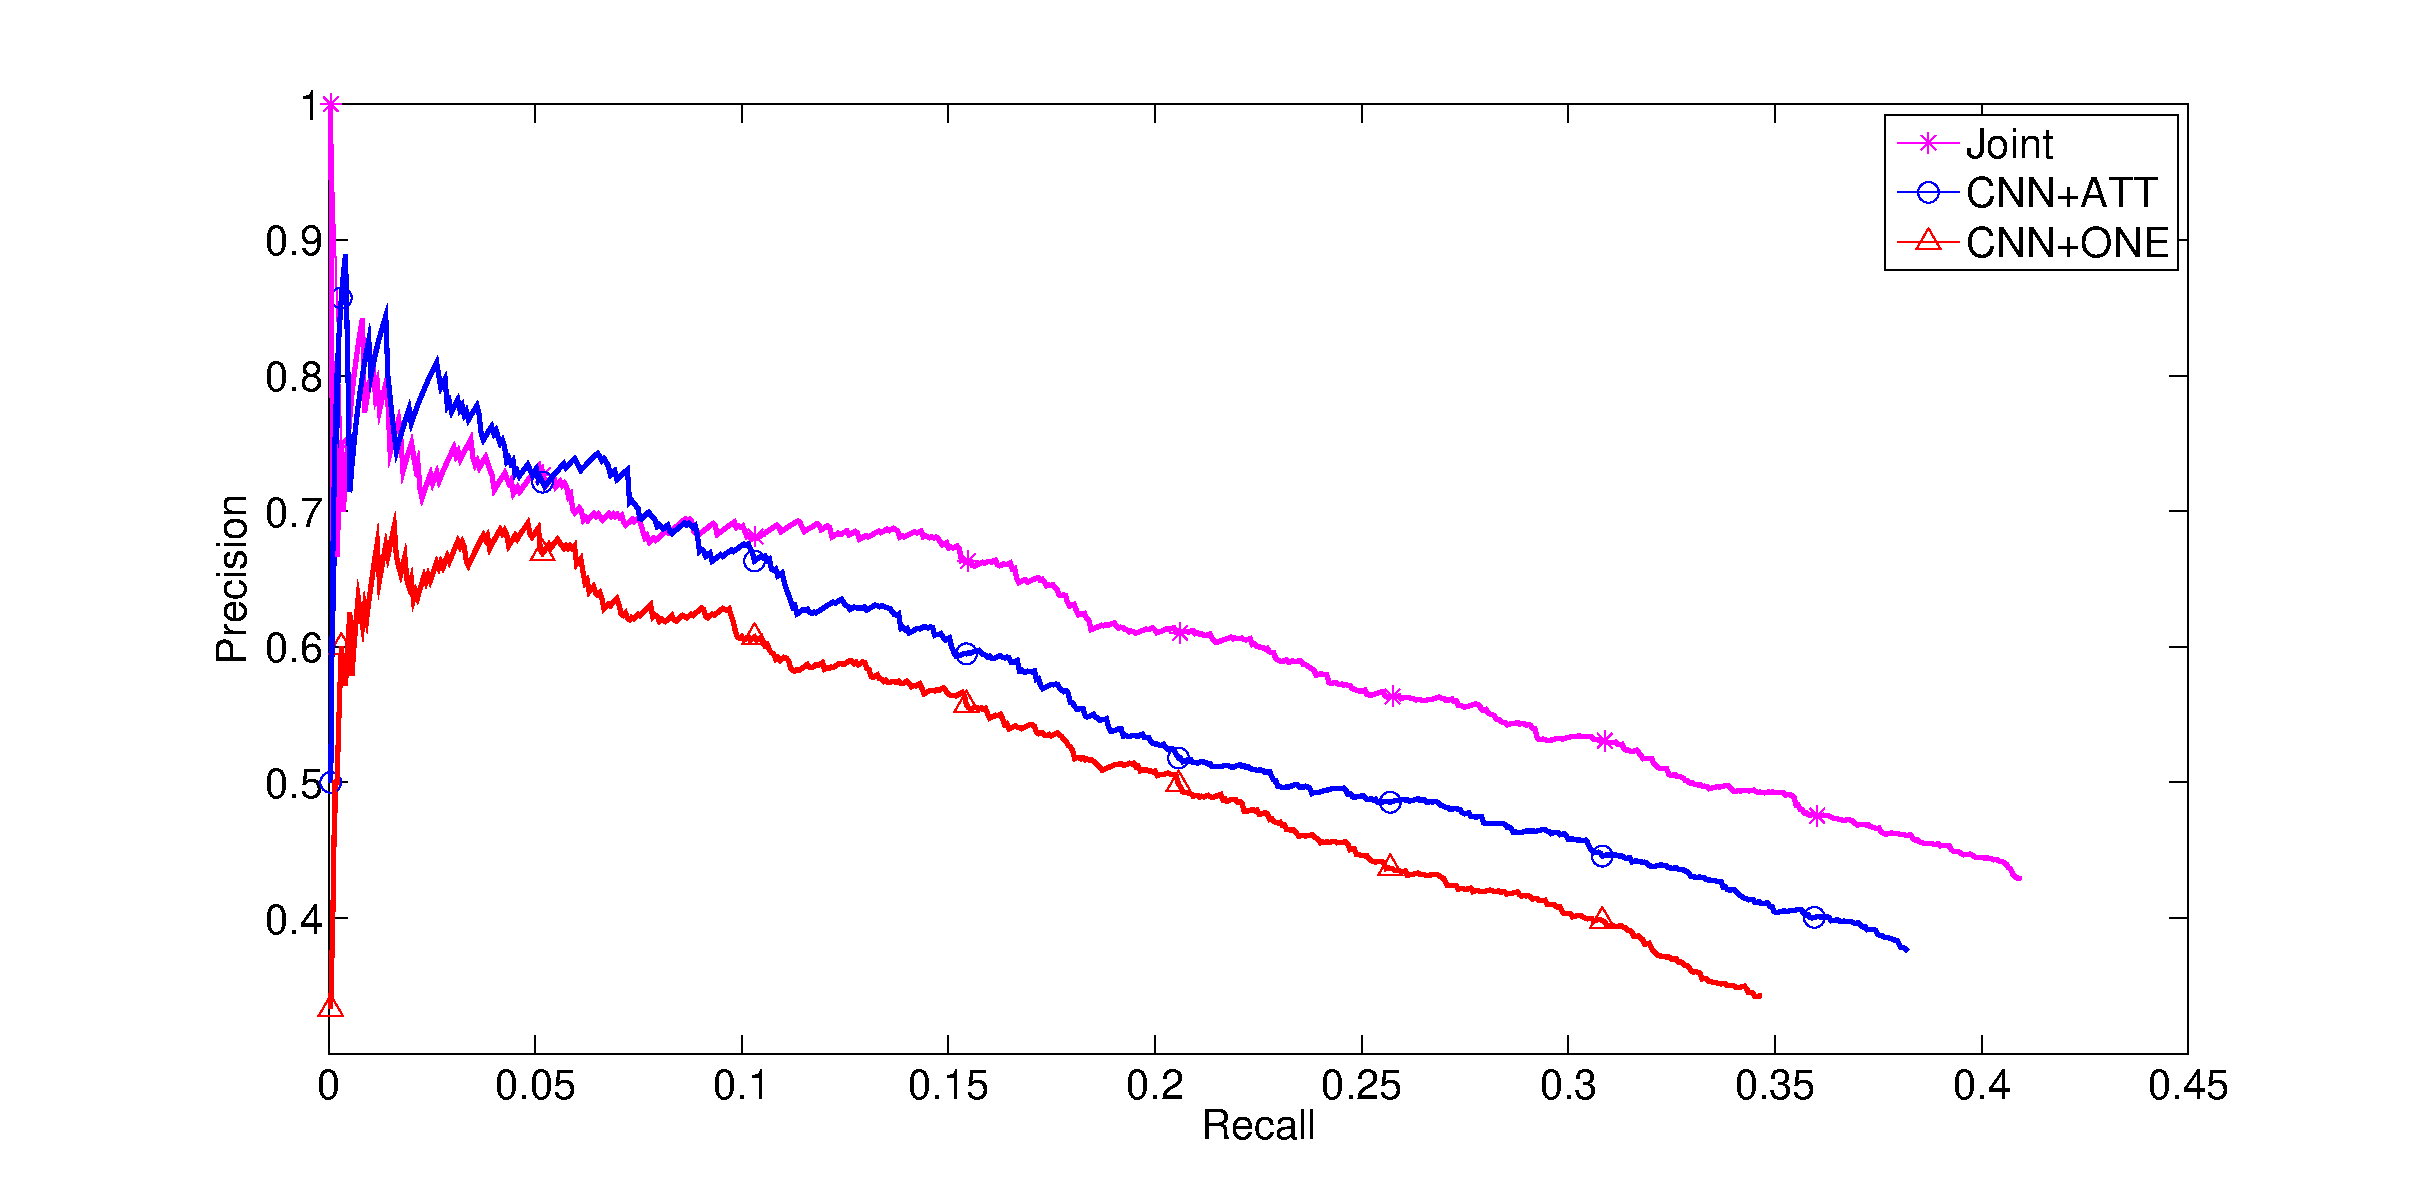
\includegraphics[width=1\columnwidth]{jointcnn.eps}
\caption{Aggregate precision/recall curves of joint learning CNN and single learning CNN.}
\label{fig:jointcnn}
\end{figure} 

We also compare our joint model with feature-based approaches, such as Mintz \cite{mintz2009distant}, MultiR \cite{hoffmann2011knowledge} and MIML \cite{surdeanu2012multi}. Mintz is a traditional distant supervised model, MultiR is a probabilistic, graphical model of multi-instance learning and MIML is a jointly model for both multiple instances and multiple relations. The results are shown in Figure \ref{fig:jointbase}


\begin{figure}[h]
% \begin{minipage}[]{0.45\linewidth}
\centering
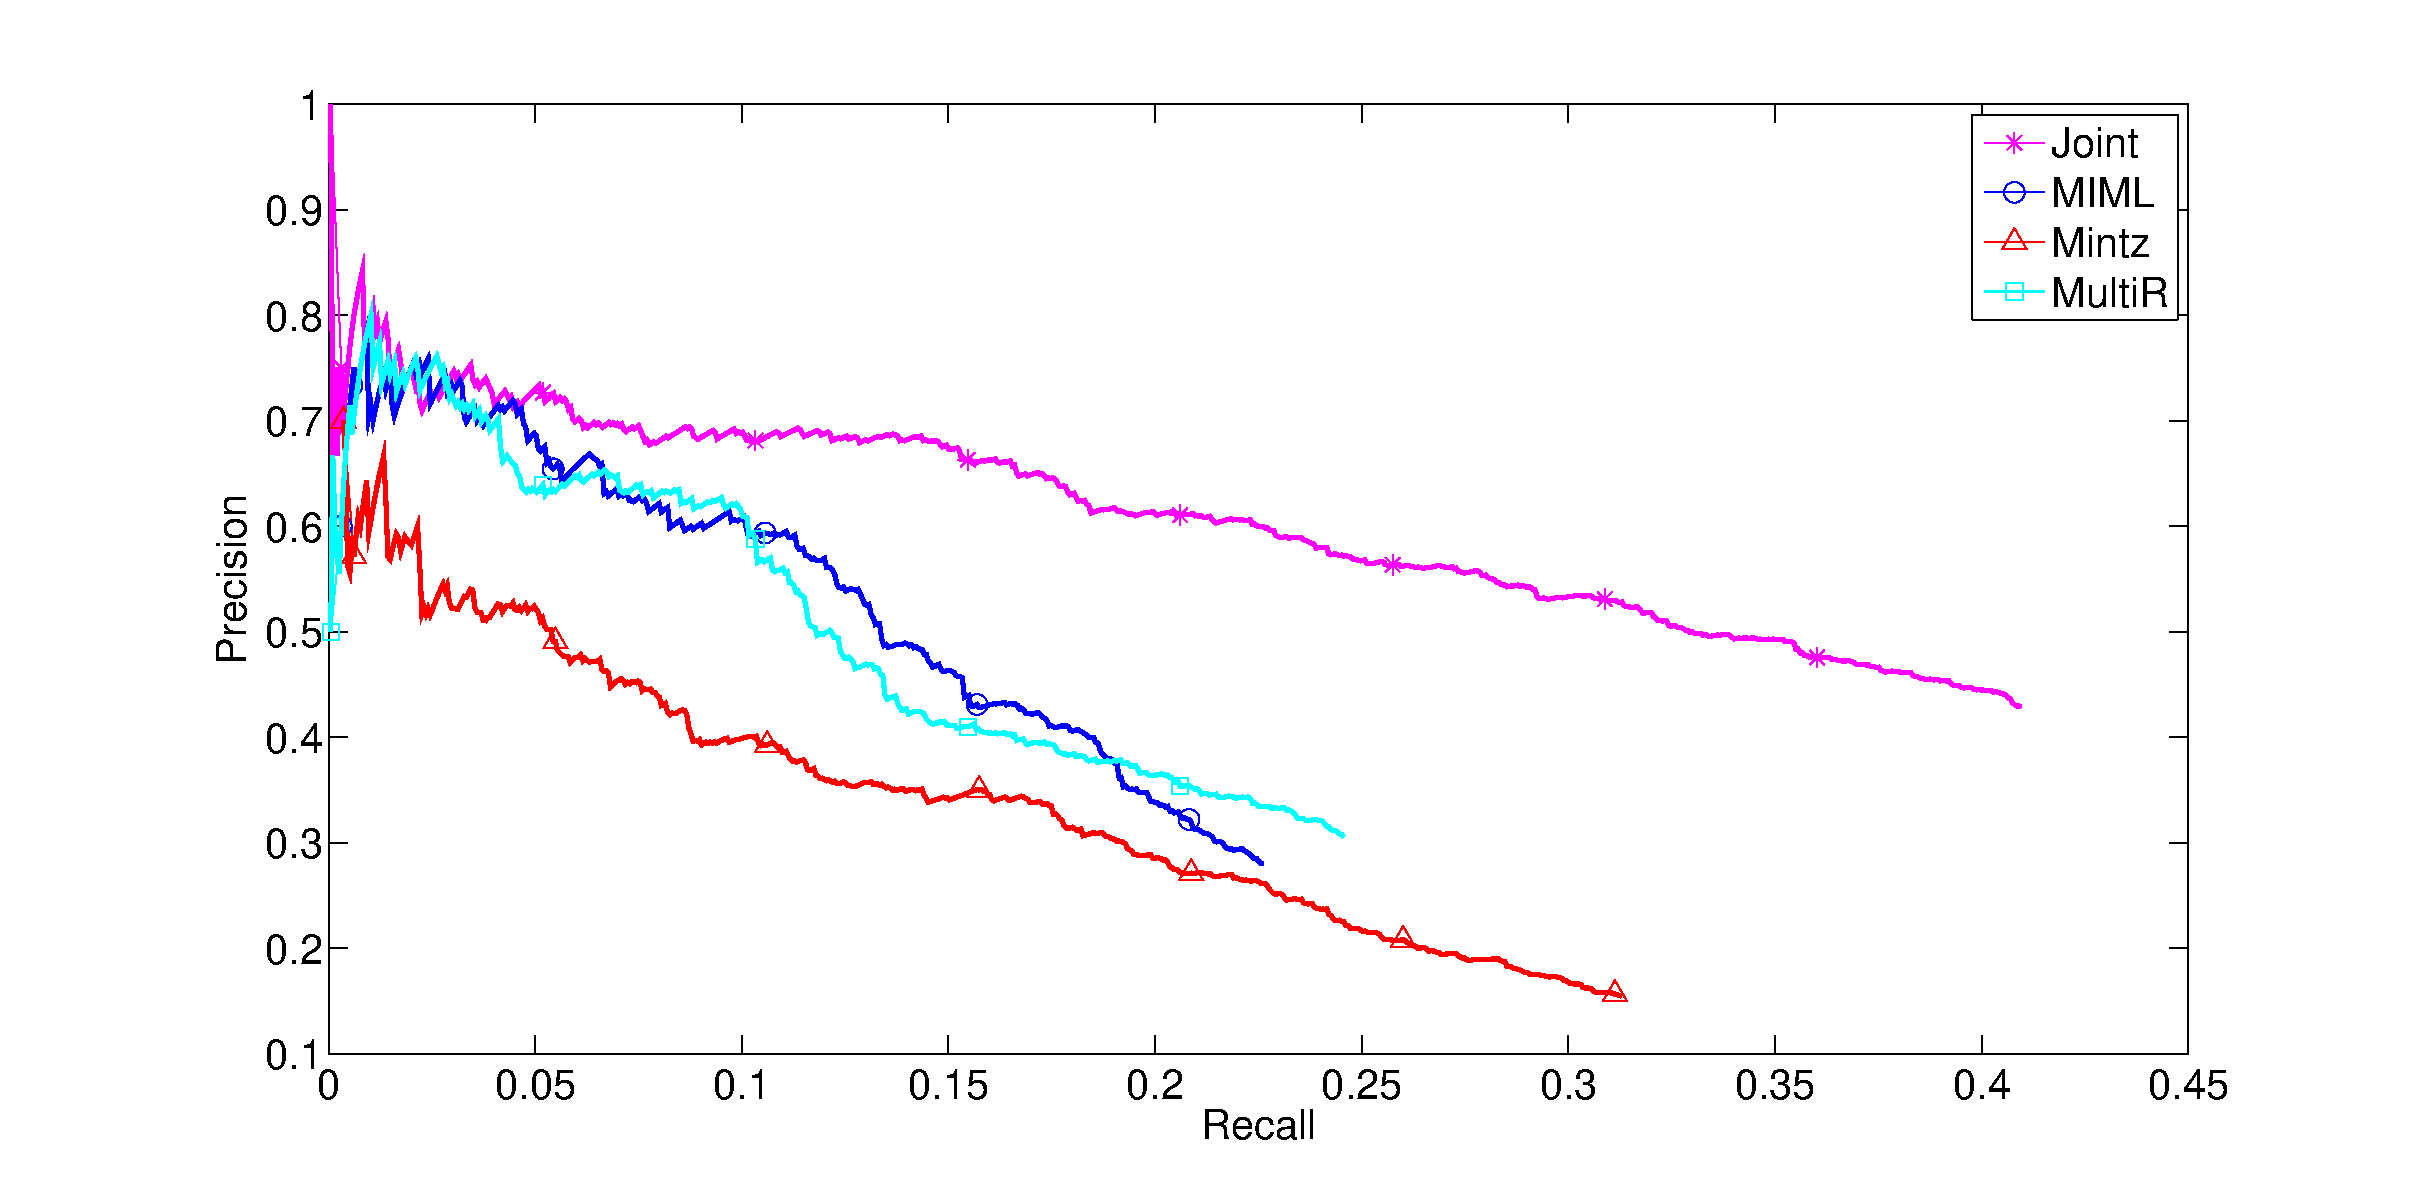
\includegraphics[width=1\columnwidth]{jointbase.eps}
\caption{Performance comparison of joint model and traditional methods.}
\label{fig:jointbase}
\end{figure} 

From the results we observe that: 

(1) The joint model get much higher prediction accuracies on the whole than CNN trained individually. It demonstrates that the joint model successfully makes use of KGs to train CNN for relation extraction. Compared to single training CNN with attention mechanism, the joint model has 5\% to 10\% improvements. These models for sentence encoding are similar, the difference of these methods are the sentence attention and the joint process. Hence, it shows that utilizing joint learning along with knowledge attention make the single model just with the sentence attention more robust. When compared to single training CNN without attention mechanism, the joint model has more amazing 10\% to 20\% improvements.

(2) Although CNN with sentence attention can achieve better performance than the joint model when the recall is small, the Joint model still significantly outperforms CNN over all the range. Features come from KGs are efficient but smooth. When knowledge features are injected into CNN via joint learning, the overall effect becomes much better along with little discrimination loss. 

(3) Compared with feature-based approaches, the joint model significantly outperforms all feature-based methods over the entire range of recall. The performance of feature-based method drop much more faster, however, the joint model has a reasonable precision even when the recall reaches $0.4$. It demonstrates that the human-designed features are limiting, though these features are structured. The knowledge features are also structured and learned by the model automatically without supervision. Hence, proposing better models to mining features is more important than designing new features for RE.


\begin{table*}[t]
\centering
\scriptsize
\begin{tabular}{|c|c|c|c|c|c|c|c|c|c|c|c|c|}
\hline
Metric            & \multicolumn{4}{c|}{Predicting Head} & \multicolumn{4}{c|}{Predicting Tail} & \multicolumn{2}{c|}{Overall} \\ \hline
                  & 1-to-1     & 1-to-N    & N-to-1    & N-to-N    & 1-to-1     & 1-to-N    & N-to-1    & N-to-N  & Triple Avg. & Relation Avg. \\ \hline

SE &35.6 &62.6 &17.2 &37.5 &34.9 &14.6 &68.3 &41.3 &39.8 & - \\ \hline
SME &35.1 &69.6 &19.9 &40.3 &32.7 &14.9 &76.0 &43.3 &41.3 & - \\ \hline
TransE            & 43.7       & 65.7      & 18.2      & 47.2      & 43.7       & 19.7      & 66.7      & 50.0    & 47.1 & - \\ \hline
TransH     & 66.8       & 87.6      & 30.2      & 64.5      & 65.5       & 39.8      & 83.3      & 67.2    & 64.4 & - \\ \hline
TransR     & 78.8       & 89.2      & 38.1      & 66.9      & 79.2       & 38.4      &\textbf{90.4}      & 72.1    & 68.7 & - \\ \hline
CTransR     & 81.5      & 89.0      & 36.4      & 71.2      & 80.8       & 38.6      &90.1      & 73.8    & 70.2 & - \\ \hline

TransD  &80.7  &85.8  &\textbf{47.1} &75.6  &80.0 &54.5 &80.7 &77.9  &74.2 &- \\ \hline


Single      & 66.5       & 88.8      & 39.8      & 79.0      & 66.4       & 51.9      & 85.6      & 81.5    & 76.6 & 66.2 \\ \hline
Joint             & \textbf{82.7}& \textbf{89.1} &45.0 & \textbf{80.7}& \textbf{81.7}& \textbf{57.7}& 87.4&\textbf{82.8} & \textbf{78.7} & \textbf{79.1} \\ \hline
\end{tabular}
\caption{Evaluation results on entity prediction of head and tail entities (\%).}
\label{t:entity}
\end{table*}


\subsection{Results of Link Prediction}

\subsubsection{Entity Prediction}

Entity prediction has also been used for evaluation in \cite{bordes2013translating,wang2014transh,lin2015learning,ji2015knowledge,he2015learning,xiao2015transg,ji2016knowledge}. More specifically, we need to predict the tail entity when given a triple $(h, r, ?)$ or predict the head entity when given a triple $(?, r ,t)$. In this task, for each missing entity, the system is asked to rank all candidate entities from the knowledge graph instead of only giving one best result. For each test triple $(h, r, t)$, we replace head and tail entities with all entities in FB15K ranked in descending order of similarity scores calculated by $\lVert \textbf{h} + \textbf{r} - \textbf{t} \rVert_2$. The relational fact $(h, r, t)$ is expected to have smaller score than any other corrupted triples.

We follow previous works and use the proportion of correct entities in Top-10 ranked entities (Hits@10) as the evaluation metric. As mentioned in \cite{bordes2013translating}, a corrupted triple may also exist in knowledge graphs, which should not be considered as incorrect. Hence, before ranking, we filter out those corrupted triples that have appeared in FB15K.

The relations in knowledge graphs can be divided into four classes: 1-to-1, 1-to-N, N-to-1 and N-to-N relations, where a ``1-to-N'' relation indicates a head entity may correspond to multiple tail entities in knowledge graphs, and so on. For example, the relation (\emph{Country}, \texttt{PresidentOf}, \emph{Person}) is a typical ``1-to-N'' relation, because there used to be many presidents for a country in history. We report the average Hits@10 scores when predicting missing head entities and tail entities with respect to different classes of relations. We also report the overall performance by averaging the Hits@10 scores over triples and over relations.

Since the evaluation setting is identical, we simply report the results of SE, SME, TransE, TransH, TransR/CTransR, TransD from \cite{bordes2011learning,bordes2012joint,bordes2013translating,wang2014transh,lin2015learning,ji2015knowledge}. The evaluation results on entity prediction is shown in Table \ref{t:entity}. The model for knowledge representation without joint learning in our framework is named as ``Single''. From Table \ref{t:entity} we observe that:

(1) The joint model almost achieves improvements under four classes of relations when predicting head and tail entities. This indicates the performance of joint learning is consistent and robust. 

(2) The improvements on ``1-to-1'', ``1-to-N'' and ``N-to-1'' relations are much more significant as compared to those on ``N-to-N''. This indicates that our joint model is more effective to embed textual relations for those deterministic relations.

(3) Our joint model achieves improvement of more than $13\%$ than Single when averaging over relations. This indicates that, our joint model can take advantages of plain texts and greatly improve representation power in relation-level.

(4) In FB15K, the relation numbers in different relation classes are comparable, but more than $80\%$ triples are instances of ``N-to-N'' relations. Since the improvement of the joint model on ``N-to-N'' relations is not as remarkable as on other relation classes, hence the overall superiority of our joint model seems not so notable when averaging over triples as compared to averaging over relations.

\subsubsection{Results of Relation Prediction}
The task aims to predict the missing relation between two entities based on their embeddings. More specifically, we need to predict the relation when given a triple $(h, ?, t)$. In this task, for each missing relation, the system is asked to find one best result, according to similarity scores calculated by $\lVert \textbf{h} + \textbf{r} - \textbf{t} \rVert_2$.
Because the number of relations is much smaller, compared with the number of entities, we use the accuracy of Top-1 ranked relations as the evaluation metric. Since some entities may have more than one relation between them, we also filter out those triples with corrupted relations appeared in knowledge graphs. We report the overall evaluation results as well as those in different relation classes.

\begin{table}[htb]
\centering
\scriptsize
\begin{tabular}{|c|c|c|c|c|c|}
\hline
Tasks             & \multicolumn{5}{c|}{Relation Prediction}                      \\ \hline
Category & 1-to-1     & 1-to-N     & N-to-1     & N-to-N     & All           \\ \hline
Single       & 24.1       & 83.0       & 80.4       & 92.5       & 87.2          \\ \hline
Joint             & \textbf{40.9} & \textbf{89.4} & \textbf{87.1} & \textbf{94.6} & \textbf{91.6} \\ \hline
\end{tabular}
\caption{Evaluation results on relation prediction (\%).}
\label{t:relation}
\end{table}

The evaluation results are shown in Table \ref{t:relation}. From Table \ref{t:relation} we observe that, our joint model outperforms Single consistently in different classes of relations and in all. The joint model also achieves more significant improvements on ``1-to-1'', ``1-to-N'' and ``N-to-1'' relations. The observations are compatible with those on entity prediction.


\section{Conclusion and Future Work}

In this paper, we propose a model for joint learning of text and knowledge representations. Our joint model embeds entities, relations and words in the same continuous latent space. More specifically, we adopt deep neural networks CNN with multilevel-attention to encode textual relations for joint learning of relation embeddings. In experiments, we evaluate our joint model on two tasks including three parts, entity prediction, relation prediction and relation extraction. Experiment results show that our joint model can effectively perform representation learning from both knowledge graphs and plain text, and obtain more discriminative entity and relation embeddings for prediction. In future, we will explore the following research directions: 

(1) The part for knowledge representation in our paper is equivalent to TransE. Our joint model is also capable to incorporate other knowledge representation models instead of TransE, such as TransH, TransR or more. In future we will explore their capability in our joint model. 

(2) We will also take more rich information in our joint model, such as relation paths in knowledge graphs, and the textual relations represented by more than one sentence in a paragraph or document. These information can also be used to incorporate into knowldege graphs.

These future work will further improve performance over knowledge and text representation, this may let the joint model make better use of knowledge and text.

\bibliography{acl2017}
\bibliographystyle{acl_natbib}

\end{document}
